\begin{lstlisting}
Section 4.7:2, 5, 8, 9 (for ed7:1,4, 8, 9)

Section 6.1:   2,  4,  6,  9,  10  (for ed7:  2,  4,  5,  8,  9)
\end{lstlisting}
\begin{exercise}
\begin{figure}[H]
\centering
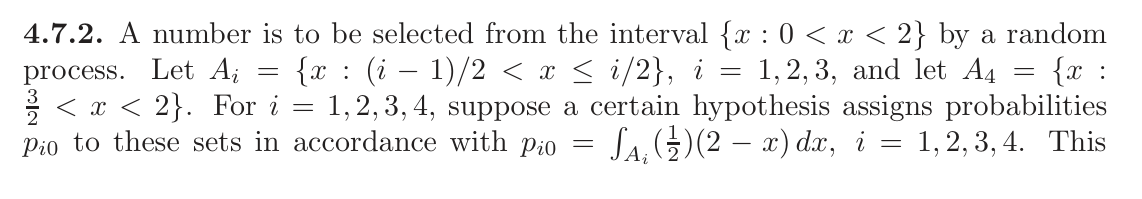
\includegraphics[width=\textwidth]{1-hw7-2025041710.png}
% \caption{}
\label{}
\end{figure}
\begin{figure}[H]
\centering
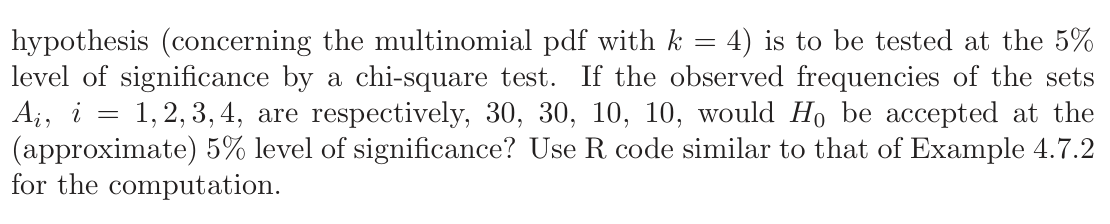
\includegraphics[width=\textwidth]{2-hw7-2025041710.png}
% \caption{}
\label{}
\end{figure}
\end{exercise}
Let $X_i$ denote the frequency of $A_i$,
\[
p_{10}=\int_{0}^{\frac{1}{2}} \frac{1}{2}(2-x) \, \mathrm{d}x =0.4375,\qquad p_{20}=\int_{\frac{1}{2}}^{1} \frac{1}{2}(2-x) \, \mathrm{d}x =0.3125
\]
\[
p_{30}=\int_{1}^{\frac{3}{2}} \frac{1}{2}(2-x) \, \mathrm{d}x =0.1875,\qquad p_{40}=\int_{\frac{3}{2}}^{2} \frac{1}{2}(2-x) \, \mathrm{d}x =0.0625
\]
\[
Q_3\coloneqq \sum_{i=1}^{4} \frac{(X_i-np_{i0})^2}{np_{i0}}\sim \chi^{2}(3)
\]
In $n=80$ trials we observe $X=(30,30,10,10)$. We will test $H_0:p=p_0$ versus $H_1:p\neq p_0$. Since $np_{10}=15$, $np_{20}=45$, $np_{30}=15$, $np_{40}=5$, the test statistic is
\[
q_3=\frac{(30-35)^2}{35}+\frac{(30-25)^2}{25}+\frac{(10-15)^2}{15}+\frac{(10-5)^2}{5}=8.38095
\]
The $p$-value is
\[
p\text{-value}=\mathbb{P}_{p_0}(Q_3\geq q_3)=\mathbb{P}_{p_0}(Q_3\geq 8.38095)=0.038761
\]
which is the smallest level at which we reject $H_0$. Since $\alpha=0.05>0.038761$, $H_0$ is rejected at $5\%$ level of significance.

\begin{lstlisting}[language=mathematica]
1 - CDF[ChiSquareDistribution[3], 8.38095]
\end{lstlisting}
\begin{exercise}
\begin{figure}[H]
\centering
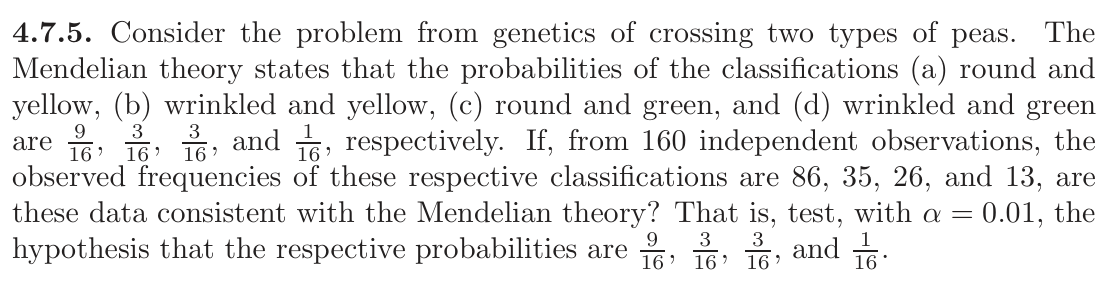
\includegraphics[width=\textwidth]{hw7-2025041711.png}
% \caption{}
\label{}
\end{figure}
\end{exercise}
The number of each type is multinomial with probability $p=\left(p_1, p_2, p_3, p_4\right)$. His theory of inheritance predicts that $p$ is equal to
\[
p_0 \equiv\left(\frac{9}{16}, \frac{3}{16}, \frac{3}{16}, \frac{1}{16}\right) .
\]
In $n=556$ trials he observed $X=(315,101,108,32)$. We will test $H_0: p=p_0$ versus $H_1: p \neq p_0$. Since, $n p_{01}=312.75, n p_{02}=n p_{03}=104.25$, and $n p_{04}=$ 34.75 , the test statistic is
\[
\begin{aligned}
\chi^2= & \frac{(315-312.75)^2}{312.75}+\frac{(101-104.25)^2}{104.25} \\
& +\frac{(108-104.25)^2}{104.25}+\frac{(32-34.75)^2}{34.75}=0.47
\end{aligned}
\]
The $\alpha=0.05$ value for a $\chi_3^2$ is $7.815$ . Since $0.47$ is not larger than $7.815$ we do not reject the null. The p-value is
\[
\text { p-value }=\mathbb{P}\left(\chi_3^2>0.47\right)=0.93
\]
which is not evidence against $H_0$.

\begin{exercise}
\begin{figure}[H]
\centering
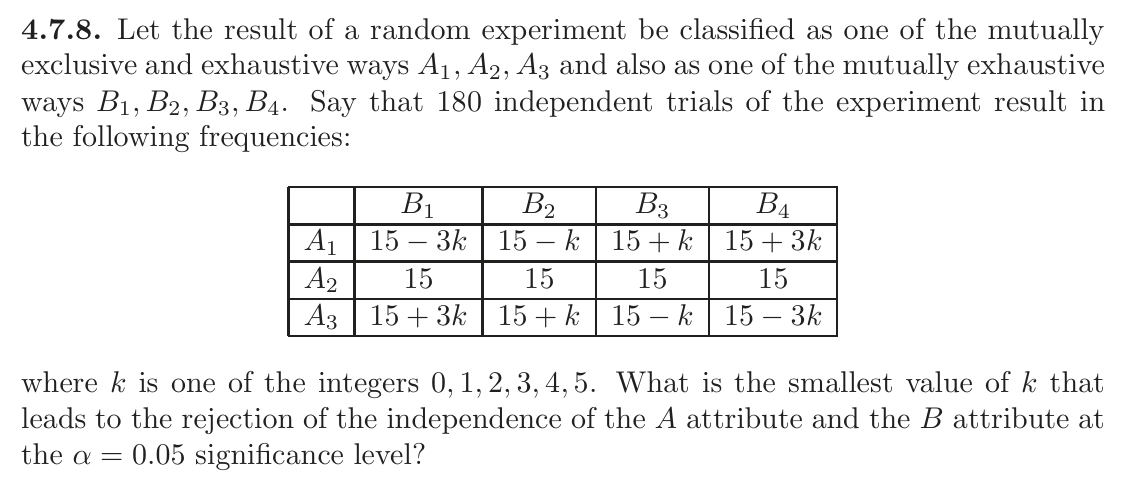
\includegraphics[width=\textwidth]{1-hw7-2025041711.png}
% \caption{}
\label{}
\end{figure}
\end{exercise}
Let $X_{ij}$ denote the frequncy of $(A_i,B_j)$, $i=1,2,3$, $j=1,2,3,4$. Let
\[
\begin{aligned}
X =( & X_{11},X_{12},X_{13},X_{14} \\
 & X_{21},X_{22},X_{23},X_{24}, \\
 & X_{31},X_{32},X_{33},X_{34})\eqqcolon (X_1,\dots,X_{12})
\end{aligned}
\]
We will test $H_0:p_{i}=\frac{1}{12},\forall i$ versus $H_1:p_{i}\neq\frac{1}{12},\forall i$. Denote
\[
Q_{11}=\sum_{i=1}^{12} \frac{(X_i-np_{i0})^2}{np_{i0}}\sim \chi^{2}(11)
\]
Fix $k\in \{ 0,1,2,3,4,5 \}$, $n=180$, then the test statistic is
\[
q_{11} = \frac{1}{15}[(3k)^2+k^2+k^2+(3k)^2+(3k)^2+k^2+k^2+(3k)^2]=\frac{8}{3}k^2
\]
\[
p\text{-value}=\mathbb{P}_{p_0}(Q_{11}\geq q_{11})=\mathbb{P}_{p_0}\left( Q_{11}\geq \frac{8}{3}k^2 \right)
\]
\[
\alpha=\mathbb{P}_{p_0}(Q_{11}\geq \chi^{2}_{11,\alpha})
\]
We reject $H_0$ at significant level $\alpha=0.05$, iff $p$ -value $\leq\alpha$, iff $\frac{8}{3}k^2\geq \chi^{2}_{11,\alpha}$, where $\chi^{2}_{11,\alpha}=19.6751$. Thus $k \geq 2.71109$. The smallest value of $k$ is $3$.

\begin{lstlisting}[language=mathematica]
alpha = 0.05;
Quantile[ChiSquareDistribution[11], 1 - alpha]
\end{lstlisting}
\begin{lstlisting}[language=mathematica]
Reduce[{8/3  k^2 >= 19.6}, k, Reals]
\end{lstlisting}
\begin{exercise}
\begin{figure}[H]
\centering
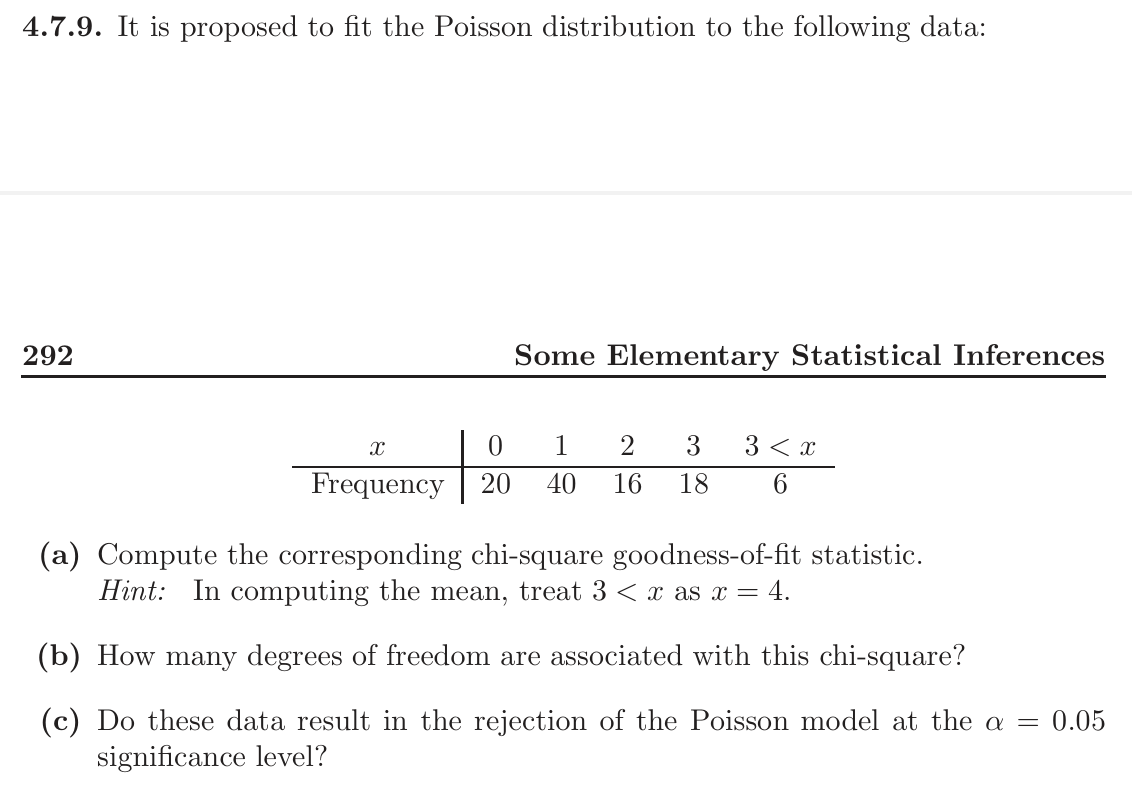
\includegraphics[width=\textwidth]{hw7-2025041712.png}
% \caption{}
\label{}
\end{figure}
\end{exercise}
Let's analyze the data and perform the chi-squared goodness-of-fit test.

The observed data is:

\begin{itemize}
	\item $x=0$: $O_0 = 20$
	\item $x=1$: $O_1 = 40$
	\item $x=2$: $O_2 = 16$
	\item $x=3$: $O_3 = 18$
	\item $x>3$: $O_4 = 6$
\end{itemize}

The total number of observations is $n = 20 + 40 + 16 + 18 + 6 = 100$.

(a) Compute the corresponding chi-square goodness-of-fit statistic.

\begin{enumerate}
	\item \textbf{Estimate the Poisson parameter $\lambda$}: As hinted, we treat the $x>3$ category as $x=4$ for computing the sample mean ($\overline{x}$), which is the estimate for $\lambda$.
\[
\widehat{\lambda} = \overline{x} = \frac{(0 \times 20) + (1 \times 40) + (2 \times 16) + (3 \times 18) + (4 \times 6)}{100}
\]\[
\widehat{\lambda} = \frac{0 + 40 + 32 + 54 + 24}{100} = \frac{150}{100} = 1.5
\]	\item \textbf{Calculate Expected Probabilities under $H_0: X \sim Poi(1.5)$}:
Using $P(X=k) = e^{-\lambda} \frac{\lambda^k}{k!}$ with $\lambda = 1.5$ ($e^{-1.5} \approx 0.22313$):
	\begin{itemize}
		\item $p_0 = P(X=0) = e^{-1.5} \approx 0.22313$
		\item $p_1 = P(X=1) = 1.5 \times e^{-1.5} \approx 0.33470$
		\item $p_2 = P(X=2) = \frac{1.5^2}{2!} e^{-1.5} \approx 0.25102$
		\item $p_3 = P(X=3) = \frac{1.5^3}{3!} e^{-1.5} \approx 0.12551$
		\item $p_{>3} = P(X \ge 4) = 1 - (p_0 + p_1 + p_2 + p_3)$
$p_{>3} \approx 1 - (0.22313 + 0.33470 + 0.25102 + 0.12551) = 1 - 0.93436 = 0.06564$
	\end{itemize}
	\item \textbf{Calculate Expected Frequencies ($E_i = n \times p_i$)}:
With $n=100$:
	\begin{itemize}
		\item $E_0 = 100 \times 0.22313 = 22.313$
		\item $E_1 = 100 \times 0.33470 = 33.470$
		\item $E_2 = 100 \times 0.25102 = 25.102$
		\item $E_3 = 100 \times 0.12551 = 12.551$
		\item $E_{>3} = 100 \times 0.06564 = 6.564$
	\end{itemize}
	\item \textbf{Calculate the Chi-Square Statistic ($\chi^2$)}:
The formula is:
\[
\chi^2 = \sum_{i} \frac{(O_i - E_i)^2}{E_i}
\]Plugging in the values:
\[
\chi^2 = \frac{(20 - 22.313)^2}{22.313} + \frac{(40 - 33.470)^2}{33.470} + \frac{(16 - 25.102)^2}{25.102} + \frac{(18 - 12.551)^2}{12.551} + \frac{(6 - 6.564)^2}{6.564}
\]\[
\chi^2 \approx \frac{(-2.313)^2}{22.313} + \frac{(6.530)^2}{33.470} + \frac{(-9.102)^2}{25.102} + \frac{(5.449)^2}{12.551} + \frac{(-0.564)^2}{6.564}
\]\[
\chi^2 \approx \frac{5.349969}{22.313} + \frac{42.6409}{33.470} + \frac{82.846404}{25.102} + \frac{29.691601}{12.551} + \frac{0.318096}{6.564}
\]\[
\chi^2 \approx 0.23976 + 1.27400 + 3.30037 + 2.36568 + 0.04846
\]\[
\chi^2 \approx 7.228
\]So, the chi-square goodness-of-fit statistic is approximately \textbf{7.228}.
\end{enumerate}

(b) How many degrees of freedom are associated with this chi-square?

The degrees of freedom ($df$) for a chi-squared goodness-of-fit test are calculated as:
\[
df = k - 1 - m
\]
Where:

\begin{itemize}
	\item $k$ = number of categories = 5 (categories are 0, 1, 2, 3, >3)
	\item $m$ = number of parameters estimated from the data = 1 (we estimated $\lambda$)
\end{itemize}

Therefore, $df = 5 - 1 - 1 = 3$.
There are \textbf{3 degrees of freedom} associated with this chi-square test.

(c) Do these data result in the rejection of the Poisson model at the $\alpha=0.05$ significance level?

\begin{enumerate}
	\item \textbf{Hypotheses}:
	\begin{itemize}
		\item $H_0$: The data follows a Poisson distribution.
		\item $H_1$: The data does not follow a Poisson distribution.
	\end{itemize}
	\item \textbf{Significance Level}: $\alpha = 0.05$.
	\item \textbf{Test Statistic}: $\chi^2 \approx 7.228$.
	\item \textbf{Degrees of Freedom}: $df = 3$.
	\item \textbf{Critical Value}: We need to find the critical value from the chi-squared distribution with 3 degrees of freedom for $\alpha = 0.05$. This is the value $\chi^2_{0.05, 3}$ such that $P(\chi^2(3) > \chi^2_{0.05, 3}) = 0.05$. Looking up this value in a chi-squared table or using statistical software:
\[
\chi^2_{0.05, 3} \approx 7.815
\]	\item \textbf{Decision Rule}: Reject $H_0$ if the test statistic $\chi^2$ is greater than the critical value $\chi^2_{0.05, 3}$.
	\item \textbf{Comparison}: $7.228 \nless 7.815$. Our test statistic is less than the critical value.
	\item \textbf{Conclusion}: Since the test statistic ($7.228$) is not greater than the critical value ($7.815$), we \textbf{fail to reject the null hypothesis ($H_0$)} at the $\alpha=0.05$ significance level.
\end{enumerate}

Therefore, based on this test, these data \textbf{do not result in the rejection} of the Poisson model at the $5\%$ significance level. There is not sufficient evidence to conclude that the data does not follow a Poisson distribution.

\begin{exercise}
\begin{figure}[H]
\centering
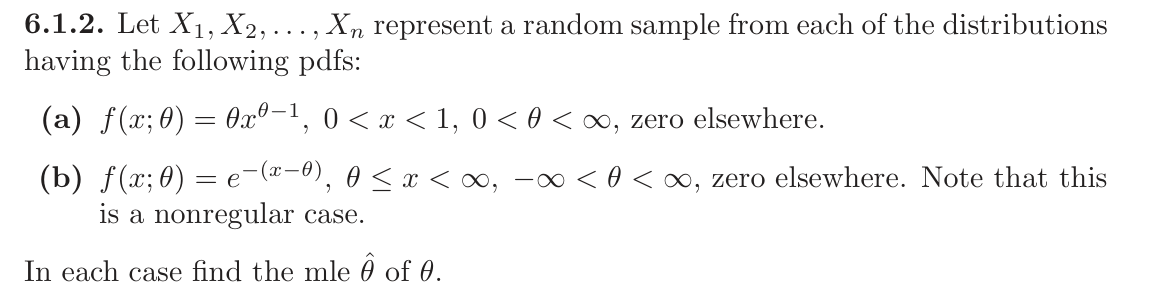
\includegraphics[width=\textwidth]{1-hw7-2025041712.png}
% \caption{}
\label{}
\end{figure}
\end{exercise}
(a)
\[
l(\theta)=\sum_{i=1}^{n} \log f(X_i;\theta)= \sum_{i=1}^{n} (\log\theta+(\theta-1)\log X_i)=n\log\theta+(\theta-1)\sum_{i=1}^{n} \log X_i
\]
Let
\[
\frac{ \partial l(\theta) }{ \partial \theta } =0
\]
i.$e$.
\[
\frac{n}{\theta}+\sum_{i=1}^{n} \log X_i=0\implies\widehat{\theta}_n=-n^{-1}\sum_{i=1}^{n} \log X_i
\]
(b)
\[
L(\theta)=\prod_{i=1}^{n} f(X_i;\theta)=\exp\left( \sum_{i=1}^{n} -(X_i-\theta)\mathbb{1}_{\{ X_i\geq \theta \}} \right)
\]
$L(\theta)$ reaches its maximum iff $\sum_{i}(X_i-\theta)\mathbb{1}_{\{ X_i\geq\theta \}}$ reaches its minimum. Thus $\widehat{\theta}_n=\min(X_1,\dots,X_n)$.

\begin{exercise}
\begin{figure}[H]
\centering
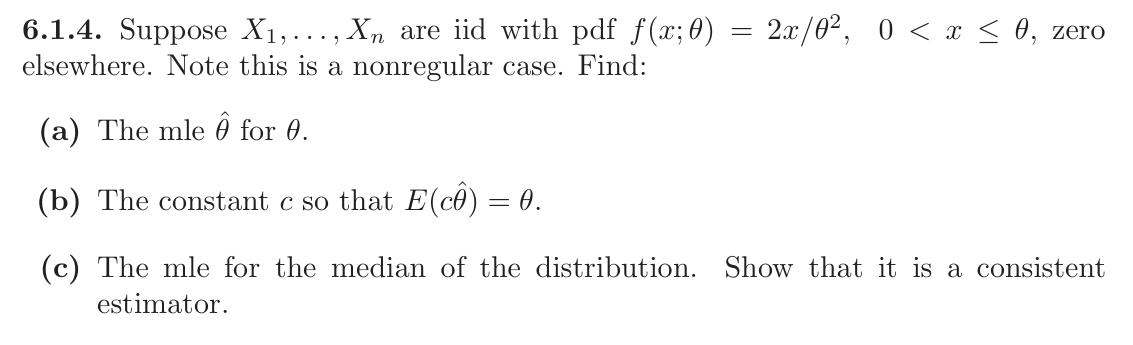
\includegraphics[width=\textwidth]{2-hw7-2025041712.png}
% \caption{}
\label{}
\end{figure}
\end{exercise}
(a)
\[
L(\theta)=\prod_{i=1}^{n} f(X_i;\theta)=\prod_{i=1}^{n} \frac{2X_i}{\theta^{2}}\mathbb{1}_{\{ 0<X_i\leq \theta \}}=\begin{cases}
\prod_{i=1}^{n} \frac{2X_i}{\theta^{2}} & \theta\geq \max_{i}(X_i) \\
0 & \theta<\max_{i}(X_i)
\end{cases}
\]
reaches its maximum at $\widehat{\theta}_n=\max_{i}(X_i)$.

(b)
Find the pdf of $\widehat{\theta}_n$.
\[
F_{\widehat{\theta}_n}(x)=\mathbb{P}(\widehat{\theta}_n\leq x)=\mathbb{P}(X_i\leq x;i=1,\dots,n)=\left( \int_{0}^{x} \frac{2t}{\theta^{2}} \, \mathrm{d}t  \right)^{n}=\left( \frac{x}{\theta} \right)^{2n}
\]
\[
f_{\widehat{\theta}_n}(x)=F'_{\widehat{\theta}_n}(x)=\theta^{-2n}\cdot2nx^{2n-1}
\]
Thus
\[
\mathbb{E}(\widehat{\theta}_n)=\int_{0}^{\theta} xf_{\widehat{\theta}_n}(x) \, \mathrm{d}x =\int_{0}^{\theta} \theta^{-2n}\cdot2nx^{2n} \, \mathrm{d}x =\frac{2n}{2n+1}\theta
\]
Therefore
\[
c=\frac{\theta}{\mathbb{E}(\widehat{\theta}_n)}=\frac{2n+1}{2n}
\]
(c)

\begin{definition}[Consistency]
Let $X$ be a random variable with cdf $F(x, \theta)$, $\theta \in \Omega$. Let $X_1, \ldots, X_n$ be a sample from the distribution of $X$ and let $T_n$ denote a statistic. We say $T_n$ is a \textbf{consistent estimator} of $\theta$ if
\[
T_n \xrightarrow{P} \theta .
\]
\end{definition}
\[
\xi_{1/2 }=F_{X_i}^{-1}(1/2 )
\]
\[
\frac{1}{2}=\int_{0}^{\xi_{1/2 }} 2x/\theta^{2} \, \mathrm{d}x=\xi_{1/2 }^2/\theta^{2}\implies \xi_{1/2 }=\frac{\theta}{\sqrt{ 2 }}
\]
By the invariance of MLE, we have
\[
\widehat{\xi_{1/2 }}=\frac{1}{\sqrt{ 2 }}\widehat{\theta}_n=\frac{1}{\sqrt{ 2 }}\max_i(X_i)
\]
Need to show that for any given $\epsilon>0$,
\[
\mathbb{P}(\lvert \widehat{\xi_{1/2 }}-\xi_{1/2 } \rvert >\epsilon)=\mathbb{P}\left(\left\lvert   \frac{1}{\sqrt{ 2 }}\max_i(X_i)-\frac{1}{\sqrt{ 2 }}\theta  \right\rvert  >\epsilon\right)\to0\qquad \text{as }n\to \infty
\]
We have
\[
\begin{aligned}
\mathbb{P}(\lvert \max_iX_i-\theta \rvert >\sqrt{ 2 }\epsilon) & =\mathbb{P}(\max_iX_i>\theta+\sqrt{ 2 }\epsilon)+\mathbb{P}(\max_iX_i<\theta-\sqrt{ 2 }\epsilon) \\
 & \overset{ 0<X_i\leq \theta,\forall i }{ = }\mathbb{P}(X_i< \theta+\sqrt{ 2 }\epsilon;\forall 1\leq i\leq n) \\
 & =\int_{0}^{\theta-\sqrt{ 2 }\epsilon} 2x/\theta^{2} \, \mathrm{d}x  ^{n} \\
 & =\left( 1-\frac{\sqrt{ 2 }\epsilon}{\theta} \right)^{2n}\longrightarrow0\qquad \text{as }n\to \infty
\end{aligned}
\]
\begin{exercise}
\begin{figure}[H]
\centering
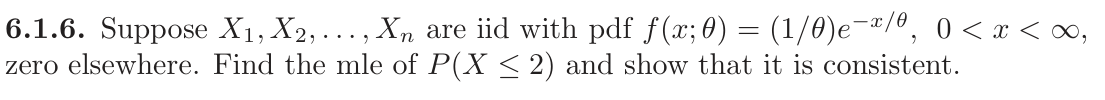
\includegraphics[width=\textwidth]{3-hw7-2025041712.png}
% \caption{}
\label{}
\end{figure}
\end{exercise}
First to find the mle of $\theta$. Let
\[
l(\theta)=\sum_{i=1}^{n} \log f(X_i;\theta)=\sum_{i=1}^{n} \left( -\frac{X_i}{\theta}-\log\theta \right)=-n\log\theta-\frac{1}{\theta}\sum_{i=1}^{n} X_i
\]
Let
\[
\frac{ \partial l(\theta) }{ \partial \theta } =0
\]
Then
\[
-n\theta ^{-1}+\theta^{-2}\sum_{i=1}^{n} X_i=0\implies\widehat{\theta}_n=n^{-1}\sum_{i=1}^{n} X_i
\]
Denote
\[
p=P(X\leq2)=\int_{0}^{2} \theta ^{-1}e^{ -x/\theta } \, \mathrm{d}x =1-e^{ -2\theta ^{-1} }
\]
Then the mle of $p$ is
\[
\widehat{p}=1-e^{ -2\widehat{\theta}_n^{-1} }=1-\exp\left( - \frac{2n}{\sum_{i=1}^{n} X_i} \right)
\]
To show $\widehat{p}$ is consistent, it suffices to show $\widehat{\theta}$ is consistent, which is consequence of the Law of Large number.

\begin{exercise}
\begin{figure}[H]
\centering
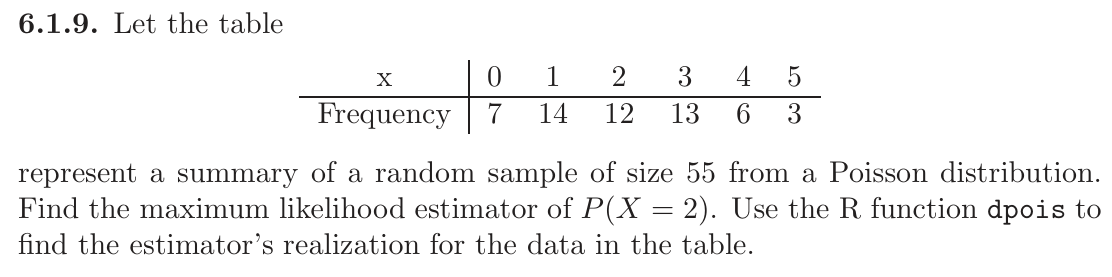
\includegraphics[width=\textwidth]{4-hw7-2025041712.png}
% \caption{}
\label{}
\end{figure}
\end{exercise}
$n=5$,
\[
\widehat{\lambda}=\sum_{k=0}^{n} \frac{k\cdot P(X=k)}{n}=\frac{0\times7+1\times14+2\times12+4\times6+5\times3}{55}=2.10909
\]
\[
p\coloneqq P(X=2)=e^{ -\lambda }\cdot\frac{\lambda^{2}}{2}
\]
Then
\[
\widehat{p}=e^{ -\widehat{\lambda} }\cdot\frac{\widehat{\lambda}^2}{2}
\]
The realization is
\[
\widehat{p}=e^{ -1.4 }\cdot\frac{1.4^2}{2}\approx 0.269895
\]
\begin{exercise}
\begin{figure}[H]
\centering
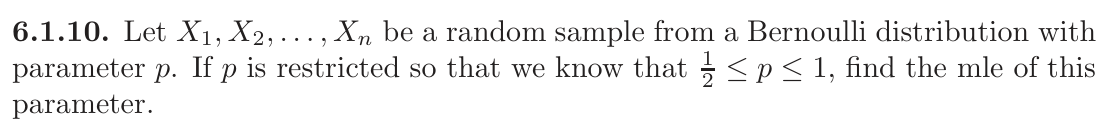
\includegraphics[width=\textwidth]{5-hw7-2025041712.png}
% \caption{}
\label{}
\end{figure}
\end{exercise}
\[
X_1,\dots,X_n\sim b(1,p)
\]
The pmf of $X$ is
\[
p(x ; p)=p^x(1-p)^{1-x}, \quad x=0 \text { or } 1 .
\]
Thus
\[
l(p)=\sum_{i=1}^{n} \log p(X_i;p)=\sum_{i=1}^{n} (X_i\log p+(1-X_i)\log(1-p))
\]
\[
\frac{ \partial l(p) }{ \partial p }= p ^{-1}\sum_{i=1}^{n} X_i-(1-p)^{-1}\left( n-\sum_{i=1}^{n} X_i \right)=0\implies \widehat{p}=n^{-1}\sum_{i=1}^{n} X_i
\]
If $n^{-1}\sum_{i=1}^{n}X_i<\frac{1}{2}$ then
\[
l(p)=\sum X_i\cdot \log p+\sum(1-X_i)\cdot \log(1-p)
\]
reaches its maximum at $p=\frac{1}{2}$, thus $\widehat{p}=\frac{1}{2}$.

If $n^{-1}\sum_{i=1}^{n}X_i\geq\frac{1}{2}$ then $\widehat{p}=n^{-1}\sum_{i=1}^{n}X_i$. Therefore
\[
\widehat{p}=\max\left( \frac{1}{2},\frac{1}{n}\sum_{i=1}^{n} X_i \right)
\]